% Kopfzeile beim Kapitelanfang:
\fancypagestyle{plain}{
%Kopfzeile links bzw. innen
\fancyhead[L]{\calligra\Large Vorlesung Nr. 22}
%Kopfzeile rechts bzw. außen
\fancyhead[R]{\calligra\Large 10.01.2013}
}
%Kopfzeile links bzw. innen
\fancyhead[L]{\calligra\Large Vorlesung Nr. 22}
%Kopfzeile rechts bzw. außen
\fancyhead[R]{\calligra\Large 10.01.2013}
% **************************************************
%
\chapter{Integration}
\sss{Idee} Sei $f:[a,b]→\R_{\geq 0}$\\*
\begin{tikzpicture}[domain=0.5:2,prefix=plots/, smooth]
\draw[very thin,color=gray] (-0.3,0.0) grid (2.5,2.0);
\draw[->] (-0.3,0) -- (2.5,0) node[right] {$x$};
\draw[->] (0,-0.3) -- (0,2) node[above] {$y$};
\draw (0.5,0) node[anchor=north] {$a$};
\draw (2,0) node[anchor=north] {$b$};
\draw[color=blue] plot[id=22.1_int1] function{sin(x)} node[below, midway] {};
\end{tikzpicture}\\*
$\int_a^b f(x)dx=$ Fläche zwischen Graphen von $f$ und $x$-Achse\\*
Wenn allgemeiner $f:[a,b]→\R$,\\*
\begin{tikzpicture}[domain=0.5:2,prefix=plots/, smooth]
\draw[very thin,color=gray] (-0.3,0.0) grid (2.5,2.0);
\draw[->] (-0.3,0) -- (2.5,0) node[right] {$x$};
\draw[->] (0,-0.3) -- (0,2) node[above] {$y$};
\draw (0.5,0) node[anchor=north] {$a$};
\draw (2,0) node[anchor=north] {$b$};
% Label zwischen Graph und X-Achse einfügen
\draw[color=blue] plot[id=22.2_int2] function{sin(2x + 0.5)} node[below, midway] {};
\end{tikzpicture}\\*
dann zählen Flächen unterhalb der $x$-Achse negativ
$$\int_a^b f(x)dx =F_1-F_2+F_3$$
\sss{Fragen}
Formale Definition des Intervalls? Welche Funktionen sind interpretierbar? Eigenschaften, Berechnung des Integrals.

\uS{Treppenfunktion}
\sS{Definition der Treppenfunktion}
Sei $a,b \eR$, $a<b$
\enum{
\item Eine Funktion $f:[a,b]→\R$ heißt Treppenfunktion, wenn es eine Unterteilung $a=x_0<x_1<x_2<x_3<…<x_n=b$ gibt, so dass $f$ auf $(x_{i-1},x_{i})$ konstant ist, dass heißt $f(x)=c_i$ für alle $x$ mit $ x_{i-1}<x<x_{i} $\\*
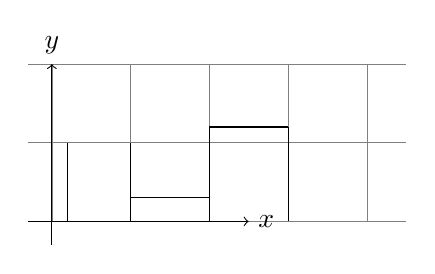
\begin{tikzpicture}
\draw[very thin,color=gray] (-0.3,0.0) grid (4.5,2.0);
\draw[->] (-0.3,0) -- (2.5,0) node[right] {$x$};
\draw[->] (0,-0.3) -- (0,2) node[above] {$y$};
% Schrafierung einfügen
\draw (0.2, 1) -- (0.2, 1);
\draw (0.2, 0) - - (0.2, 1);
\draw (1, 0) - - (1, 1);
\draw (1, 0.3) -- (2, 0.3);
\draw (2, 0) - - (2, 1.2);
\draw (2, 1.2) -- (3, 1.2);
\draw (3, 0) - - (3, 1.2);
\end{tikzpicture}
\item In diesem Fall definiere
$$\int_a^b f(x)dx=\sum_{i=1}^n c_i(x_{i}-x_{i-1})$$
"Summe der Rechtecke"
\bem
Die Definition eines Integrals für die Treppenfunktion ist unabhängig von der Unterteilung
\bsp
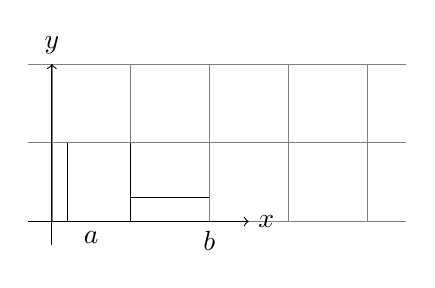
\begin{tikzpicture}
\draw[very thin,color=gray] (-0.3,0.0) grid (4.5,2.0);
\draw[->] (-0.3,0) -- (2.5,0) node[right] {$x$};
\draw[->] (0,-0.3) -- (0,2) node[above] {$y$};
\draw (0.5,0) node[anchor=north] {$a$};
\draw (2,0) node[anchor=north] {$b$};
% Schrafierung einfügen
\draw (0.2, 1) -- (0.2, 1);
\draw (0.2, 0) - - (0.2, 1);
\draw (1, 0) - - (1, 1);
\draw (1, 0.3) -- (2, 0.3);
\end{tikzpicture}\\*
(ohne formalen Beweis)
}

\sS{Lemma}
Seien $f,g:[a,b]→\R$ Treppenfuntionen\\*
Dann gilt:
\enum{
\item $\ds\int_a^b (f+g)(x)dx=\int_a^b f(x)dx+\int_a^b g(x)dx$
\item $\ds c\eR \int_a^b c·f(x)dx=c·\int_a^b f(x)dx$
\item Wenn $f\leq g$, dass heißt $f(x)\leq g(x)\ ∀x$, dann $\ds \int_a^b f(x)dx\leq \int_a^b g(x)dx$\\*
\begin{tikzpicture}[domain=0.5:2,prefix=plots/, samples=10]
\draw[very thin,color=gray] (-0.3,0.0) grid (2.5,2.0);
\draw[->] (-0.3,0) -- (2.5,0) node[right] {$x$};
\draw[->] (0,-0.3) -- (0,2) node[above] {$y$};
\draw[color=blue] plot[id=22.5_x3const, const plot] function{-(x-2)**3} node[below, midway] {};
\draw[color=red] plot[id=22.5_x3] function{-(x-2)**3} node[below, midway] {};
\end{tikzpicture}\\*
(ohne formalen Beweiß)
}

\uS{Das Riemannsche Integral}
\ul{Idee} Sei $f: [a, b] \to \R$ beliebige Funktion.\\*
Wenn $g \leq f$ und $g$ Treppenfunktion dann sollte $\int g(x)dx < \int f(x)dx$
Wenn $f \leq h$ und $f$ Treppenfunktion dann sollte $\int f(x)dx < \int h(x)dx$
Wenn $\int^b_a f(x)dx$ durch diese ($\infty$-vielen) Bedingungen festgelegt wird, nennen wir $f$ integrierbar und $\int_a^b f(x) dx$ ist definiert.

\sS{Definition des Riemannschen Integral}
Sei $f:[a,b]→\R$ beschränkte Funktion\\*
Unterintegral:
$$sup \left\{\int_a^b g(x)dx\mid g:[a,b]\text{ Treppenfunktion mit }g\leq f\right\}=:\int_a^b{}_* f(x)dx$$
Oberintegral:
$$inf \left\{\int_a^b h(x)dx\mid h:[a,b]\text{ Treppenfunktion mit }f\leq h\right\}=:\int_a^b{}^* f(x)dx$$
(\ul{Idee} Wenn $\int_a^b f(x)$ definiert, sollte $ \int_a^b{}_* f(x)dx\leq \int_a^b f(x)dx \leq \int_a^b{}^* f(x)dx $)
\sss{Definition}
$f$ heißt integrierbar, wenn $\int_a^b{}_* f(x)dx=\int_a^b{}^* f(x)dx$\\*
Dann setzte $\int_a^b f(x)dx:=\int_a^b{}_* f(x)dx$

\sS{Bemerkung}
$f:[a,b] \to \R$ ist integrierbar \equ{} es gilt: Für jedes \e > 0 gibt es eine Treppenfunktion $g,\ h$ mit $g \leq f \leq h$ mit $\int_a^b h(x)dx - \int_a^b g(x)dx < \e$. Damit ist $\int_a^b f(x)$ auf $\e$ festgelegt.

\sS{Satz Eigenschaften des Integrals}
Seien $f, g: [a, b] \to \R$ integrierbar, dann sind auch $f + g$ und $c \cdot f$ integrierbar und
\enum{
\item $\int_a^b (f + g)(x) dx = \int_a^b f(x) + \int_a^b g(x)$
\item $\int_a^b (c \cdot f)(x) dx = c \cdot \int_a^b f(x)$
\item wenn $f \leq g$ dann $\int f(x)dx \leq \int g(x)dx$
}
\bew
\notat{$I(f) = \int f(x)dx$}
Sei $\e > 0$ gegeben.\\*
Wähle Treppenfunktion $f_1, f_2, g_1, g_2$ mit $f_1 < f < f_2$ und $g_1 < g < g_2$\\*
$I(f_2) - I(f_1) < \e$, $I(g_2) - I(g_1) < \e$\\*
\Larr{} $f_1 + g_1 < f + g < f_2 + g_2$\\*
%Lustige Pfeile
$I(f_2 + g_2) - I(f_1 + g_1) = I(f_2) - I(f_1) + I(g_2) - I(g_1) < \e + \e = 2\e$\\*
Das für jedes $\e > 0$ \\*
$|I(f + g) - I(f) - I(g)| \leq |I(f + g) - I(f_1 + g_1)| + |I(f) - I(f_1)| + |I(f) - I(f_1)| = 2\e + \e + \e = 4\e$\\*
(Dreiecksungleichung)\\*
\Rarr{} $I(f + g) - I(f) - I(g) = 0$\\
Rest des Satzes analog. \qed{}

\sS{Satz}
Sei $f:[a,b]→\R$ stetig, dann:
\enum{
\item Für jedes $ε>0$ gibt es eine Treppenfuntion $g:[a,b]→\R$ mit $|f(x)-g(x)|<ε$ für alle $x\in[a,b]$\\*
\begin{tikzpicture}[domain=0.5:2,prefix=plots/, smooth]
\draw[very thin,color=gray] (-0.3,0.0) grid (2.5,2.0);
\draw[->] (-0.3,0) -- (2.5,0) node[right] {$x$};
\draw[->] (0,-0.3) -- (0,2) node[above] {$y$};
\draw[color=blue] plot[id=22.6_x3const, const plot, samples=10] function{(0.3x-2)**2} node[below, midway] {};
\draw[color=red] plot[id=22.6_x3] function{(0.3x-2)**2} node[below, midway] {};
\end{tikzpicture}
\item $f$ ist integrierbar
}
\bew
Zeige 2) unter Annahme von 1).\\*
Gegeben $ε>0$. Setze $ε'=\frac{1}{2(b-a)}ε$\\*
Wegen 1) gibt es eine Treppenfunktion $g:[a,b]→\R$ mit $|f(x)-g(x)|<ε'$.
$$g_1(x)=g(x)-ε',\ g_2(x)=g(x)+ε'\ \Rarr\ g_1\leq f \leq g_2$$
\alg{&\int_a^b g_2(x)dx-\int_a^b g_1(x)dx=\int_a^b (g_2-g_1)(x)dx=\int_a^b \underset{\overset{\uparrow}{konstante\ Funktion}}{2ε'}(x)dx\\*
&={2ε'}(b-a)=\frac{1}{(b-a)}·ε·2(b-a)=ε\ \underset{9.4}{\Rarr} f\text{integrierbar}}
Zeige \enum{
\item Gegeben sei $\e > 0$\\
6.24 \Rarr{} $f$ gleichmäßig aber stetig. d.h. es gibt $\delta > 0$ so dass gilt:\\*
Wenn $|x-y|<\delta$ dann $|f(x) - f(y)|<\e$\\*
Wähle Unterteilung $a = x_0 < x_1 < x_2 < ... < x_n = b$ mit $x_i - x_{i-1} < \delta$
%Graph
Sei $c := f(x_i)$ \\*
Definiere Treppenfunktion $g:[a,b] \to \R$\\*
$x_{i-1} < x < x_i$ \Rarr{} $g(x) = c_i = f(x)\ (1 \leq i \leq n)$\\*
$g(x_0) = f(x_0)$ dann $|f(x) - g(x)| < \e$ für alle $x$.\qed{}
}

\sS{Satz (Mittelwertsatz der Integralrechnung)}
Sei $f:[a,b]→\R$ stetig (somit integrierbar)\\*
Dann gibt es ein $x_0\in [a,b]$ mit $\ds\int_a^b f(x)dx=f(x_0)(b-a)$\\*
GRAPH
\bew
\desc{Sei}{$m=inf{f(x)\mid x\in [a,b]}$\\$M=sup{f(x)\mid X\in [a,b]}$}
6.11 \Rarr\ \ul{Bekannt} es gibt $x_1,x_2\in [a,b]$ mit $f(x_1)=m,f(x_2)=M$\\*
$f(x_1)\leq f(x_2)$ für alle $f(x)\leq f(x_2)$
\Rarr{} $f(x_1)(b-a) = \int_a^b f(x) \leq \int_a^b dx \leq_a^bf(x_2) dx = f(x_2)(b-a)$\\*
$f(x_1) \leq \frac{1}{b-a} \int_a^b f(x)dx \leq f(x)$\\*
Zwischenwertsatz \Rarr{} es gibt auch $x_0 \in [a, b]$ mit $f(x_0) = y$ \Rarr{} $f(x_0)(b-a) = \int_a^b f(x)dx$

(nachtrag)
\sS{Definition Mittelwertsatz}
Sei $f:[a,b]→\R$ integrierbar, $a<b$
$$\int_b^a f(x)dx=-\int_a^b f(x)dx$$
\sss{Konsequenz}
Sei $f:I→\R$ stetig $a,b,c\in I$, dann $$\int_a^b f(x)dx+\int_b^c f(x)dx=\int_a^c f(x)dx$$ egal wie $a,b,c$ liegen!\\*
WEITERE Graphen